\documentclass{beamer}

\usepackage[brazilian]{babel}
\usepackage[T1]{fontenc}
\usepackage[utf8]{inputenc}
\usepackage{default}

\usetheme{Hannover}

\setbeamertemplate{caption}[numbered]

\title{Sistema de Compartilhamento de Livros}
\author{Amilcar Machado Júnior \and Marcelo Garlet Millani}
\institute{Instituto de Informática}

\begin{document}

\begin{frame}{}
 \maketitle 
\end{frame}

\section{Realidade}

\begin{frame}{Universo}
 
 \begin{itemize}
  \item Usuários se organizam em grupos
  \item Cada membro oferece um livro
  \item Os membros trocam livros entre si
 \end{itemize}
 
 \end{frame}
 
 \section{Sistema}
\begin{frame}{Propósito do Sistema}
	\begin{itemize}
	 \item Permitir a organização de grupos públicos e privados
	 \item Determinar um ciclo de trocas de forma que todos os membros recebam todos os livros (e o dono receba o seu de volta)
	 \item Proteger a anonimidade dos usuários o máximo possível 
	\end{itemize}
\end{frame}

\section{Diagramas}

\begin{frame}{Componentes} 
 \begin{figure}
  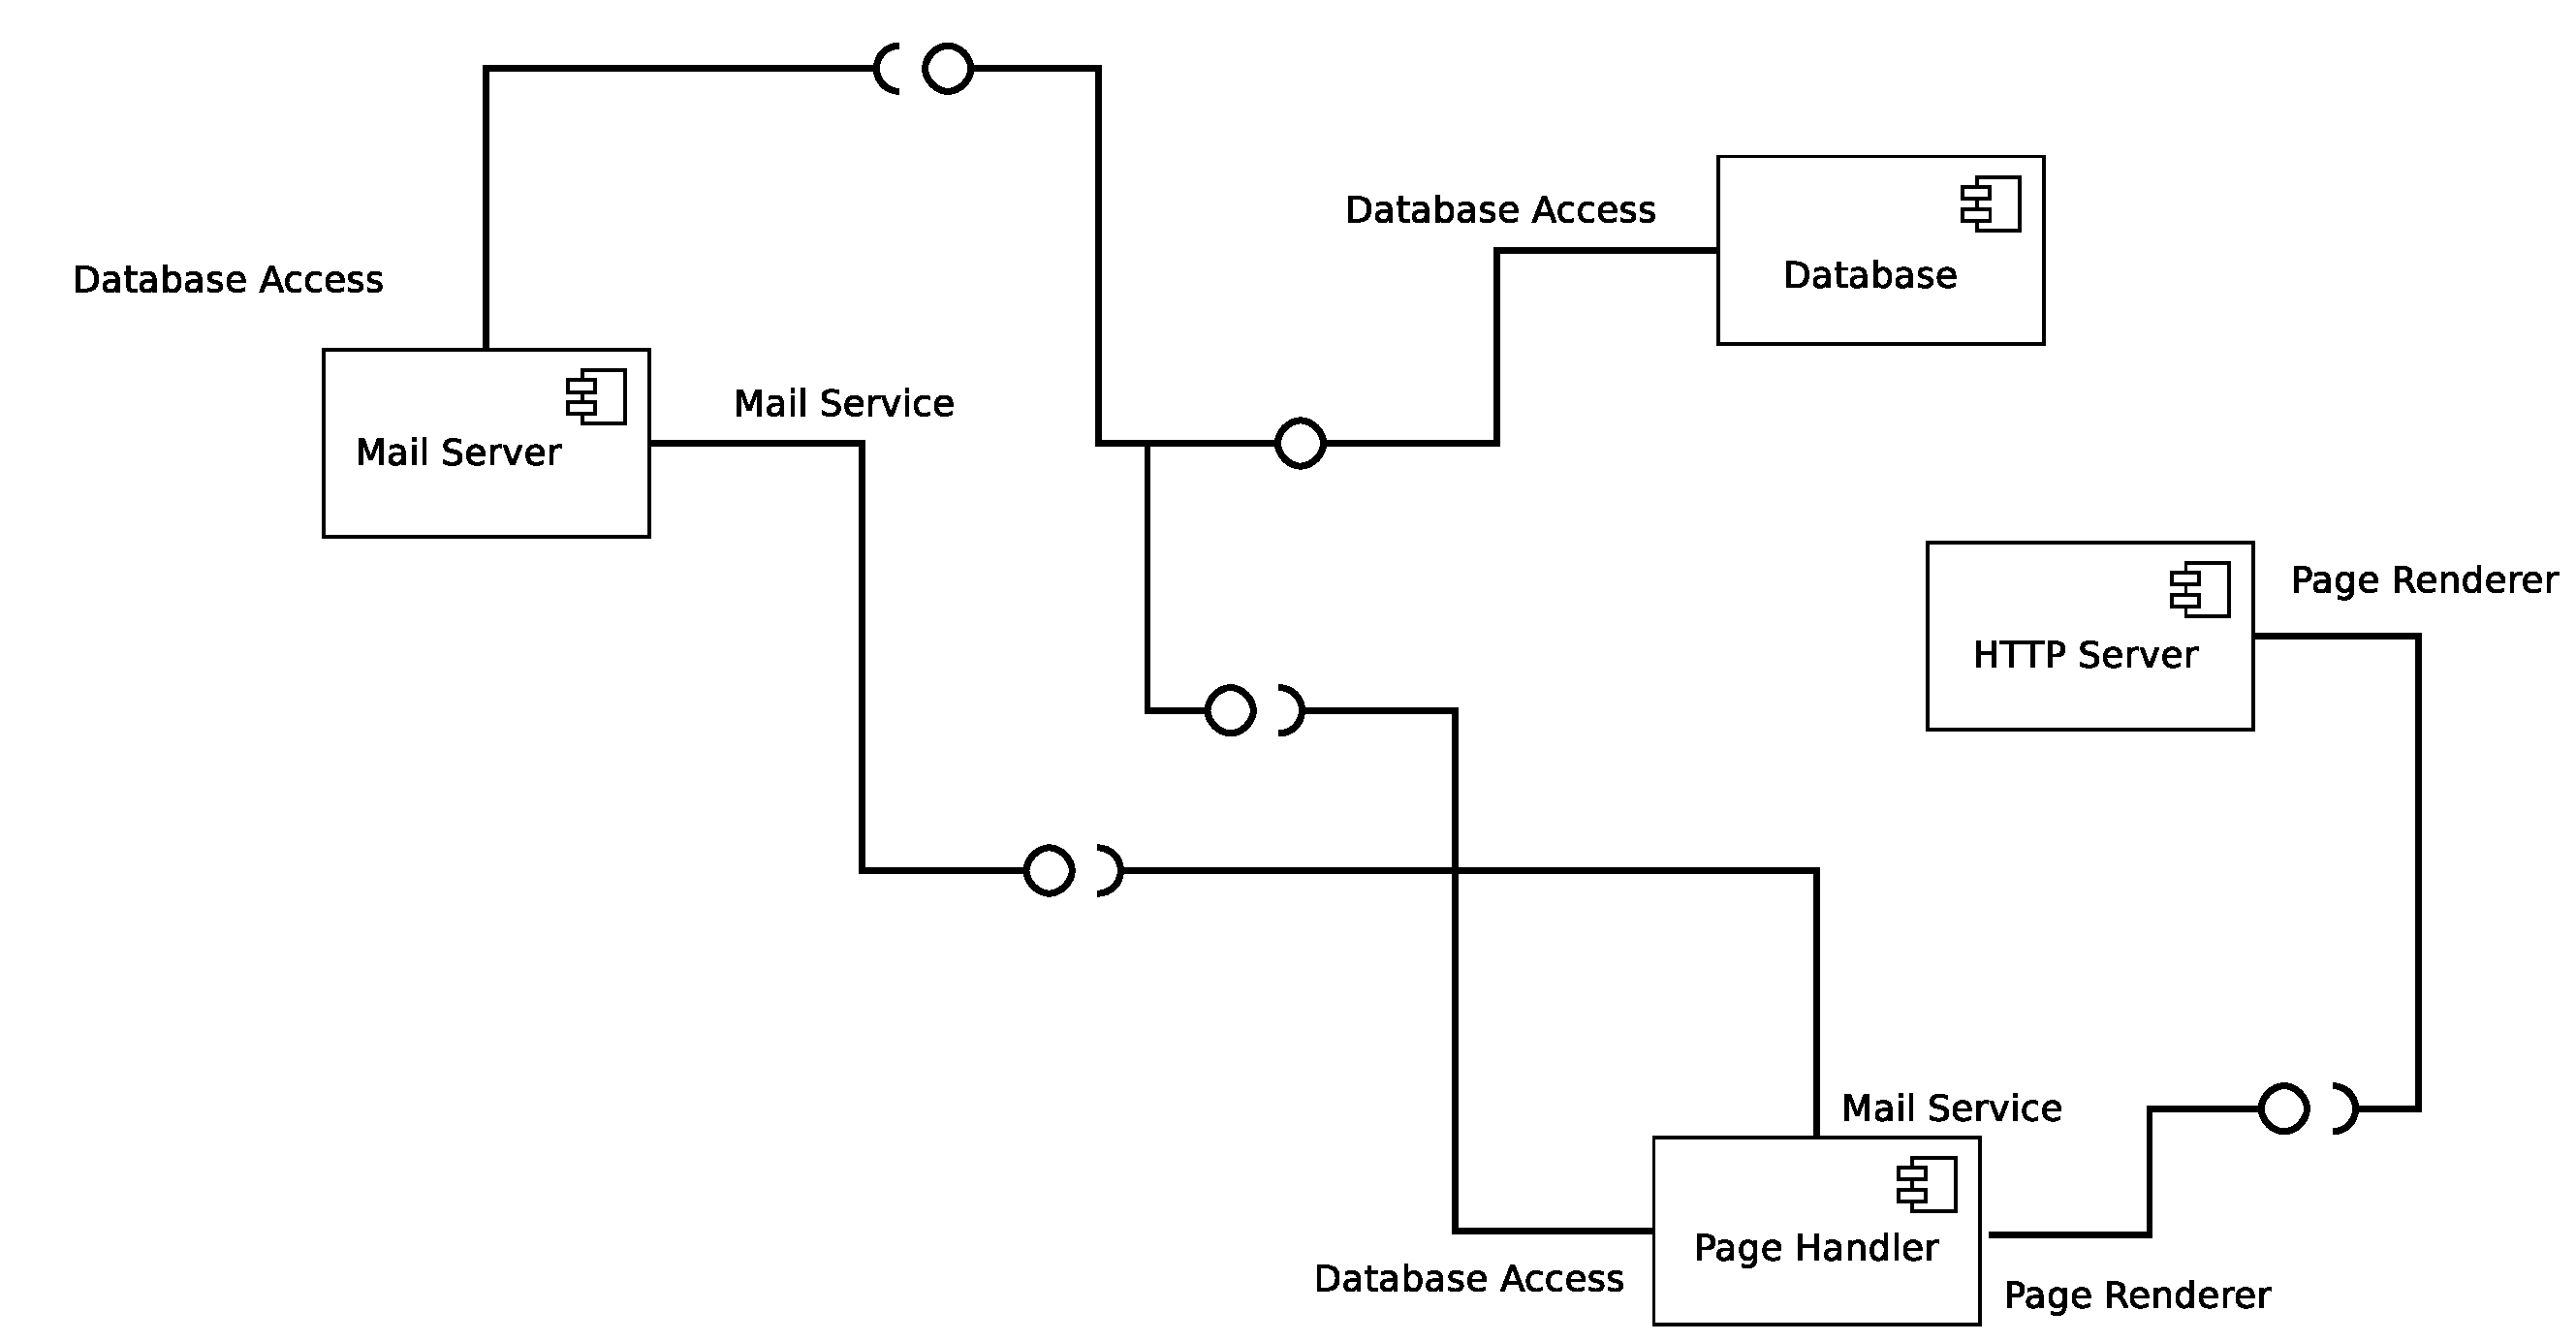
\includegraphics[width=\textwidth]{componentes.eps}
  \caption{Diagrama de Componentes}  
 \end{figure} 
\end{frame}

\begin{frame}{Pacotes}
 \begin{figure}
  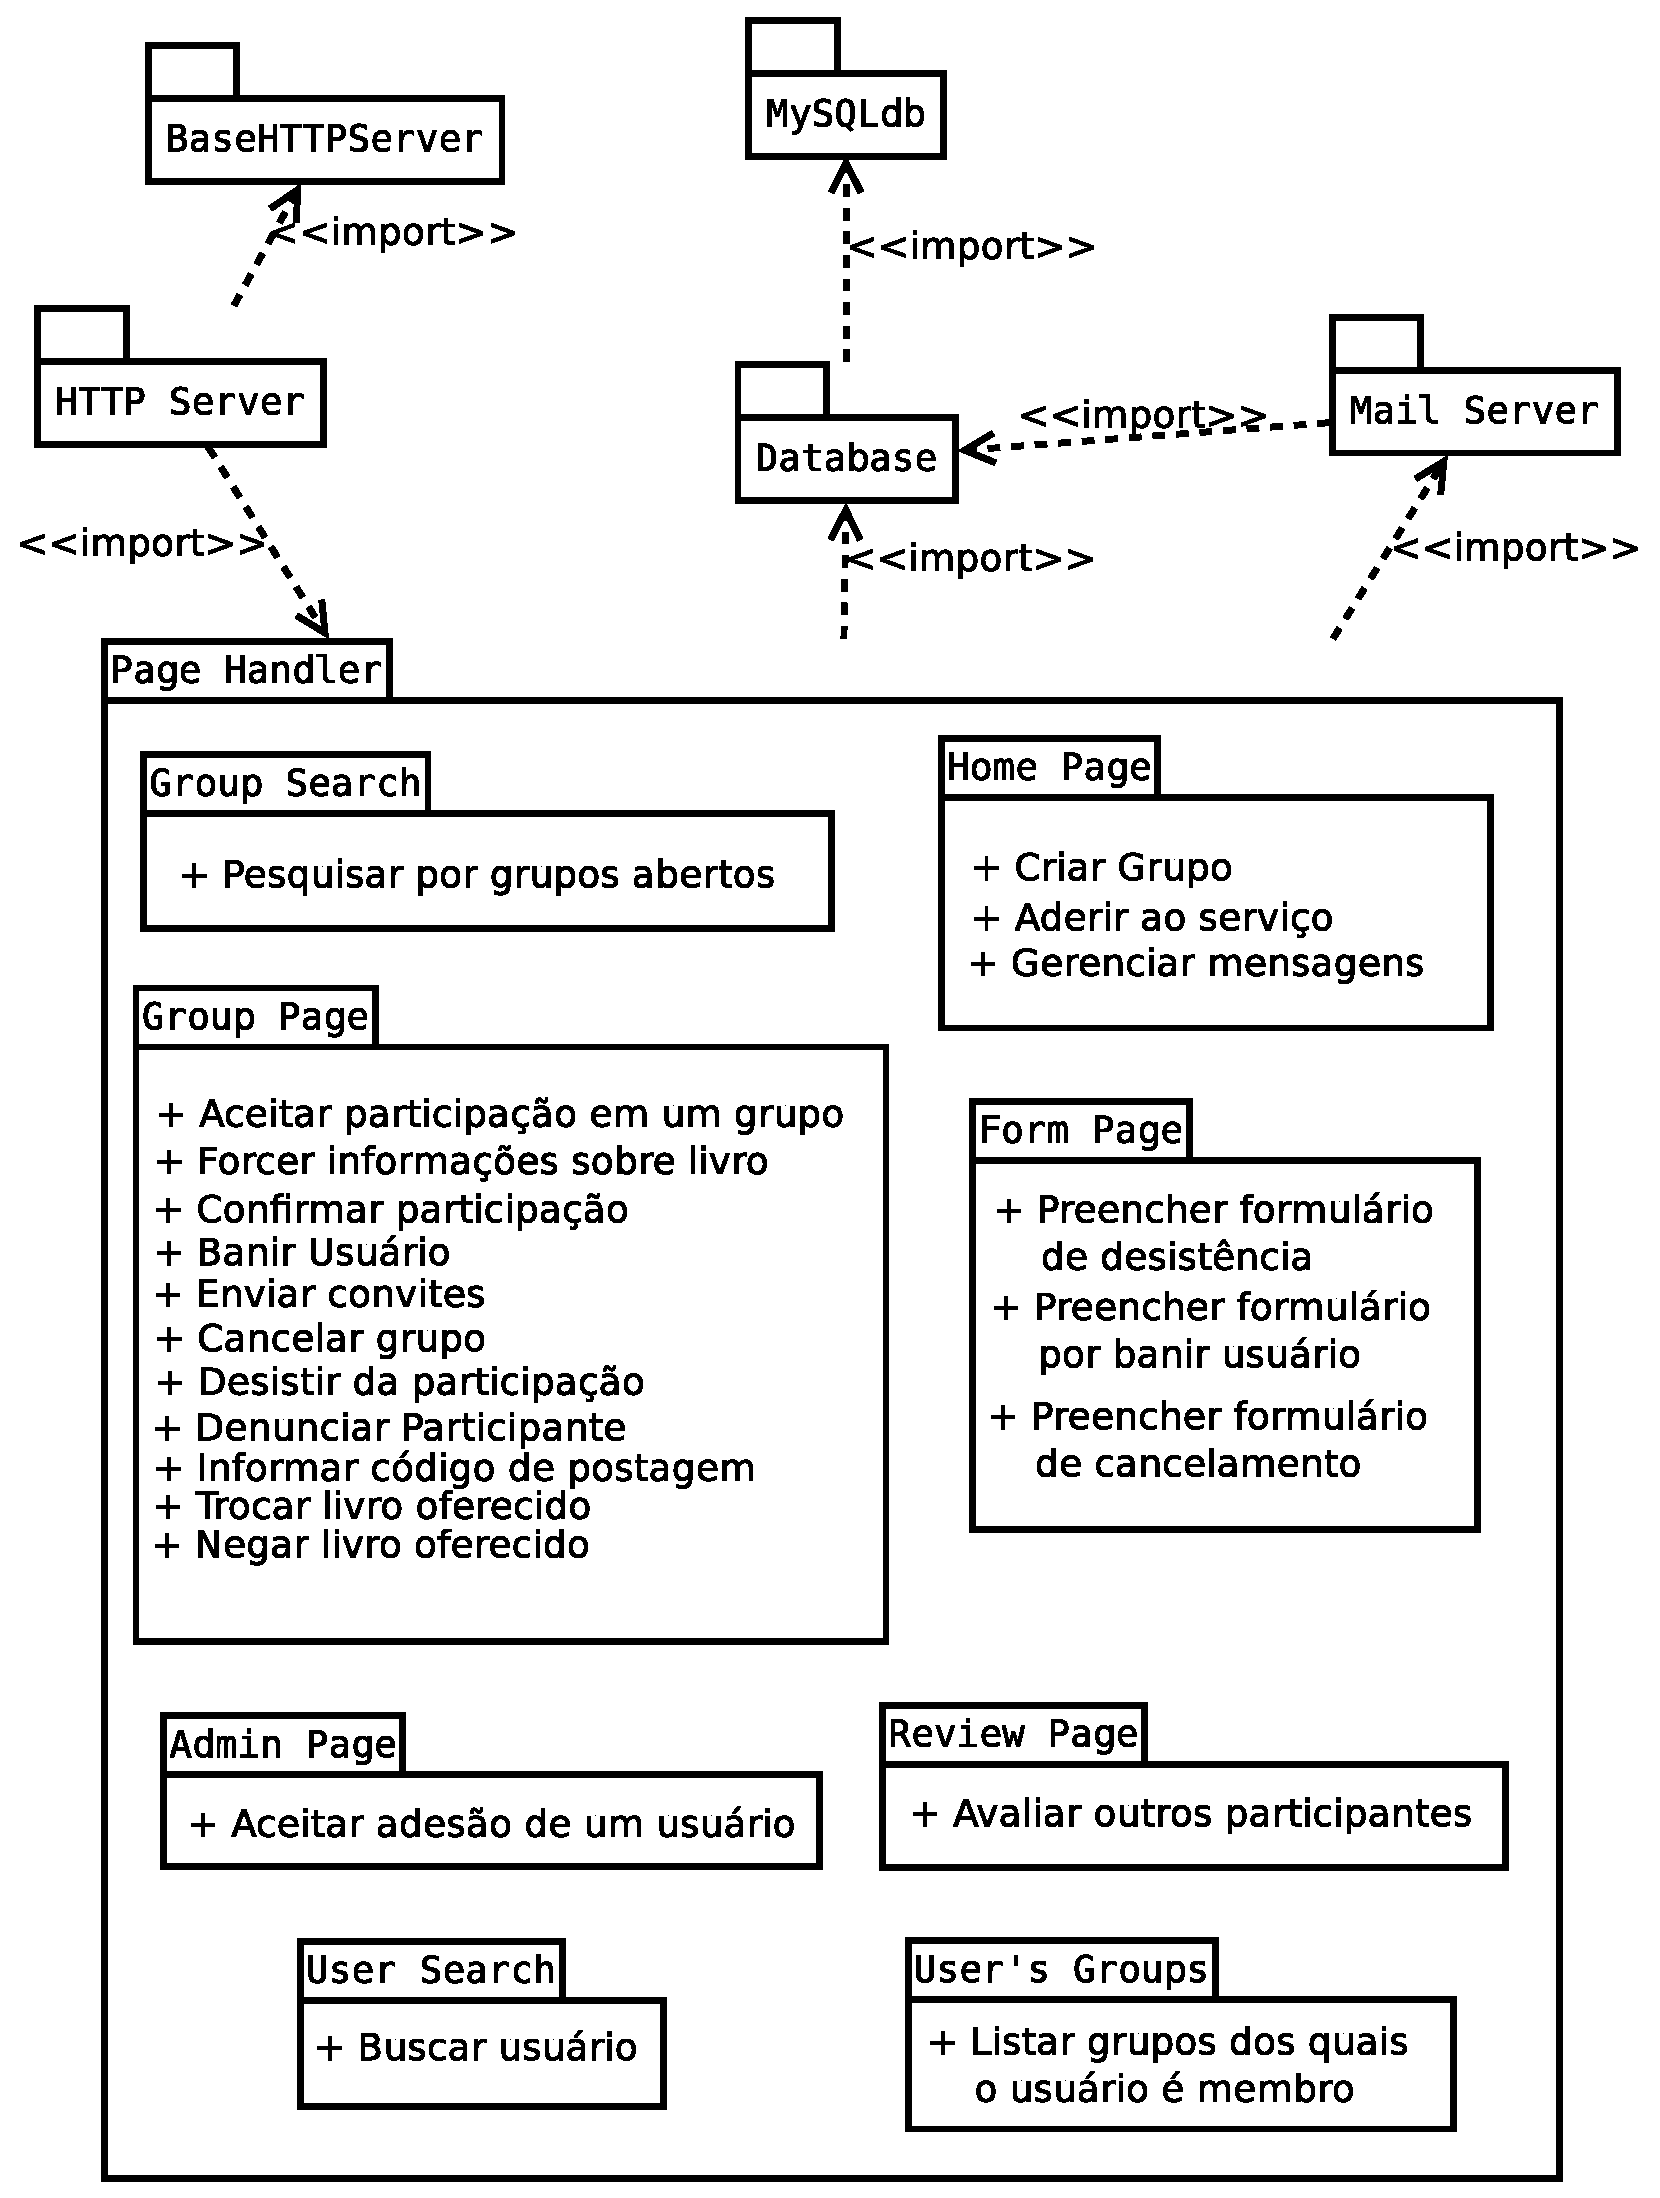
\includegraphics[height=0.7\textheight]{pacotes.eps}
  \caption{Diagrama de Pacotes}  
 \end{figure} 
\end{frame}

\begin{frame}{Modelo ER}
 \begin{figure}
  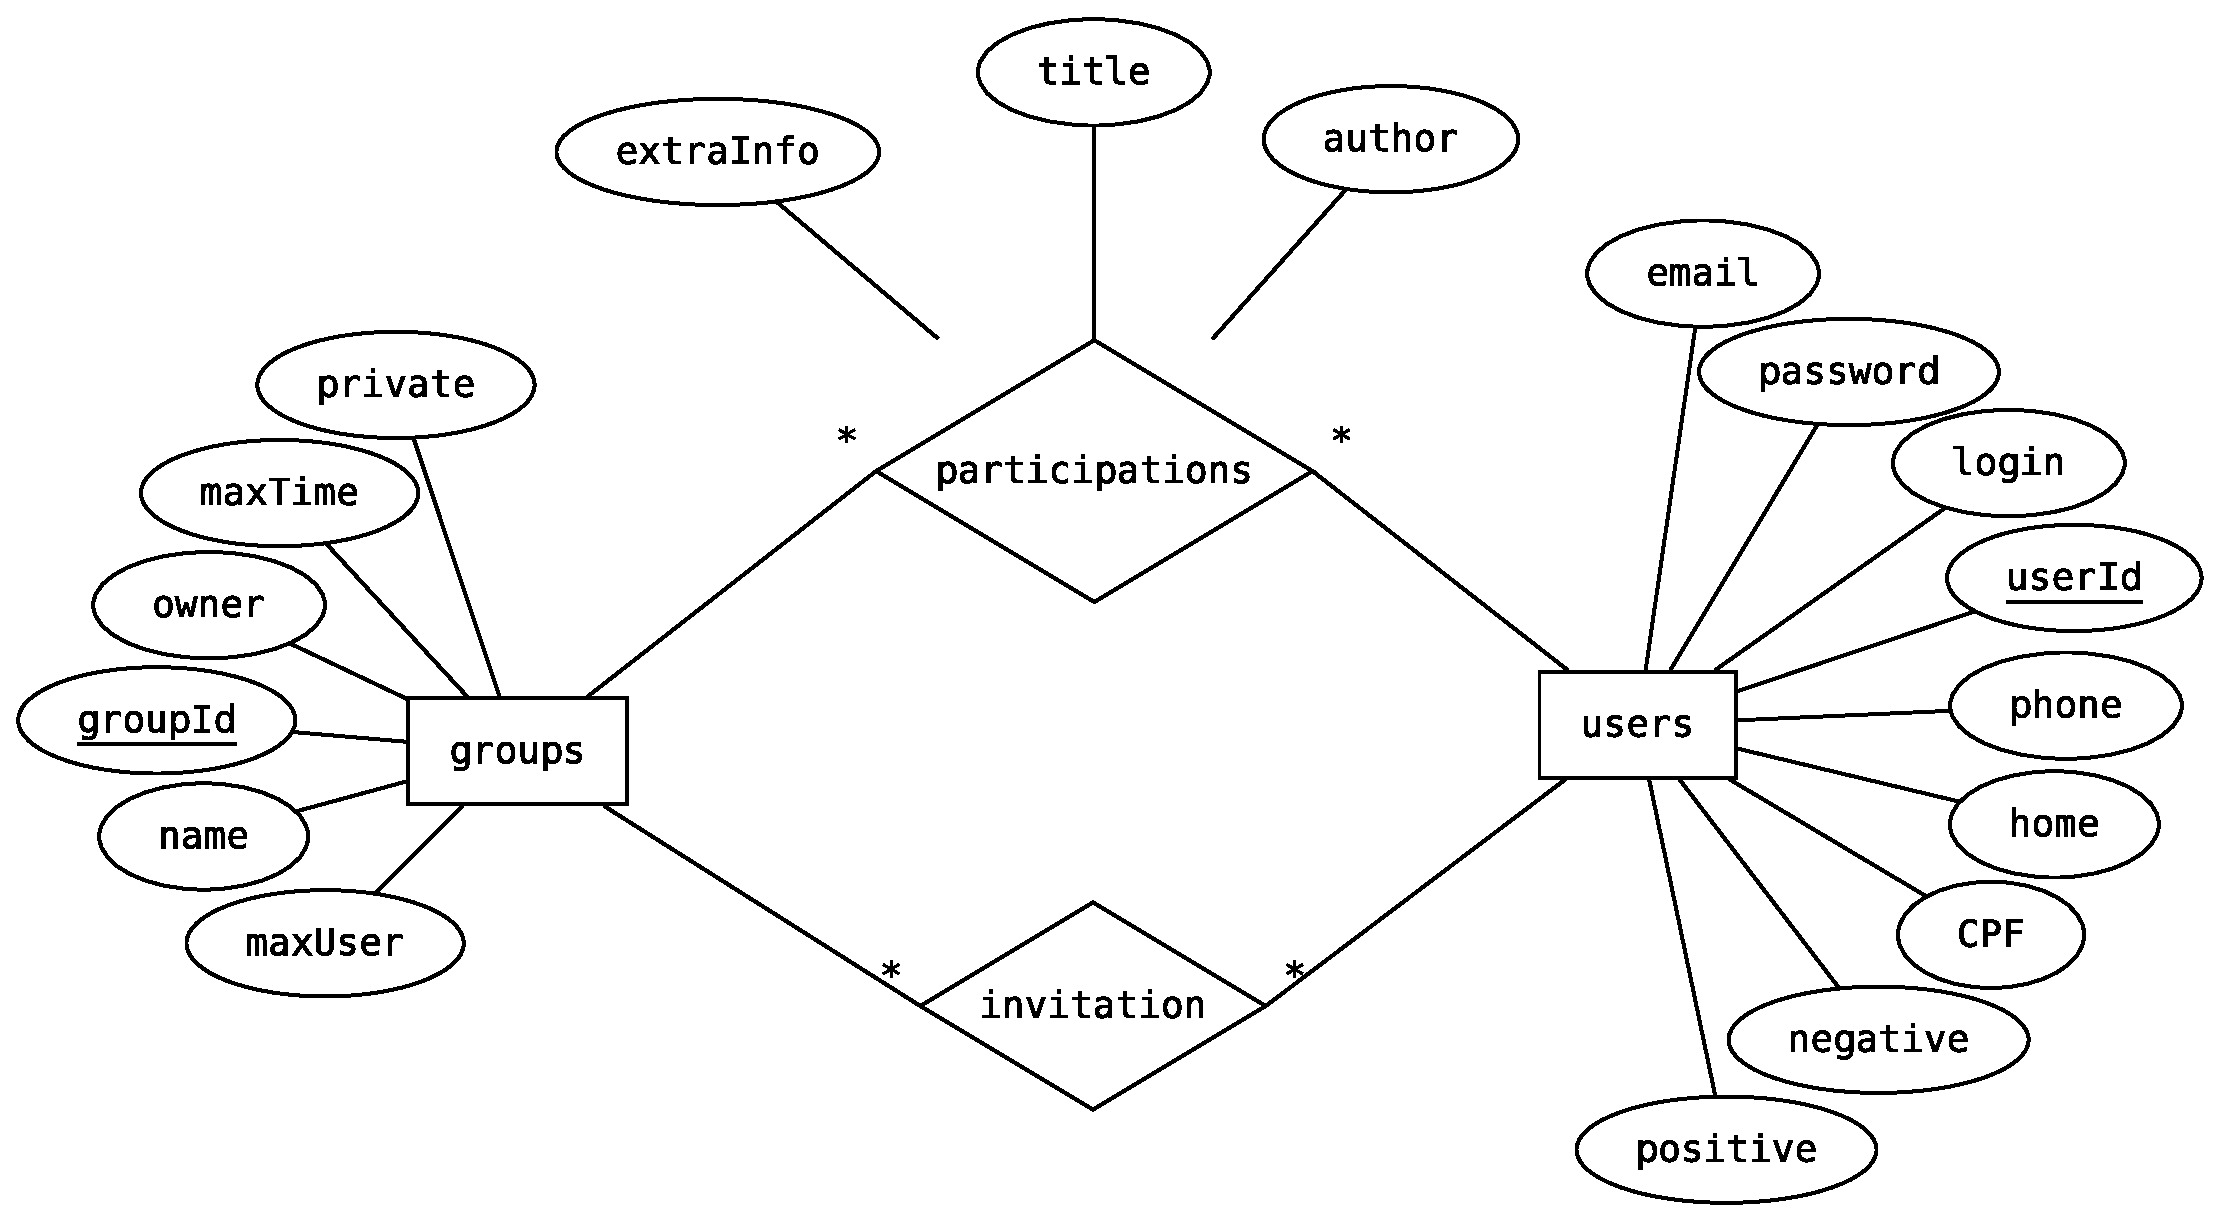
\includegraphics[width=\textwidth]{modeloER.eps}
  \caption{Modelo Entidade-Relacionamento}  
 \end{figure} 
\end{frame}

\begin{frame}{Casos de Uso}
 \begin{figure}
  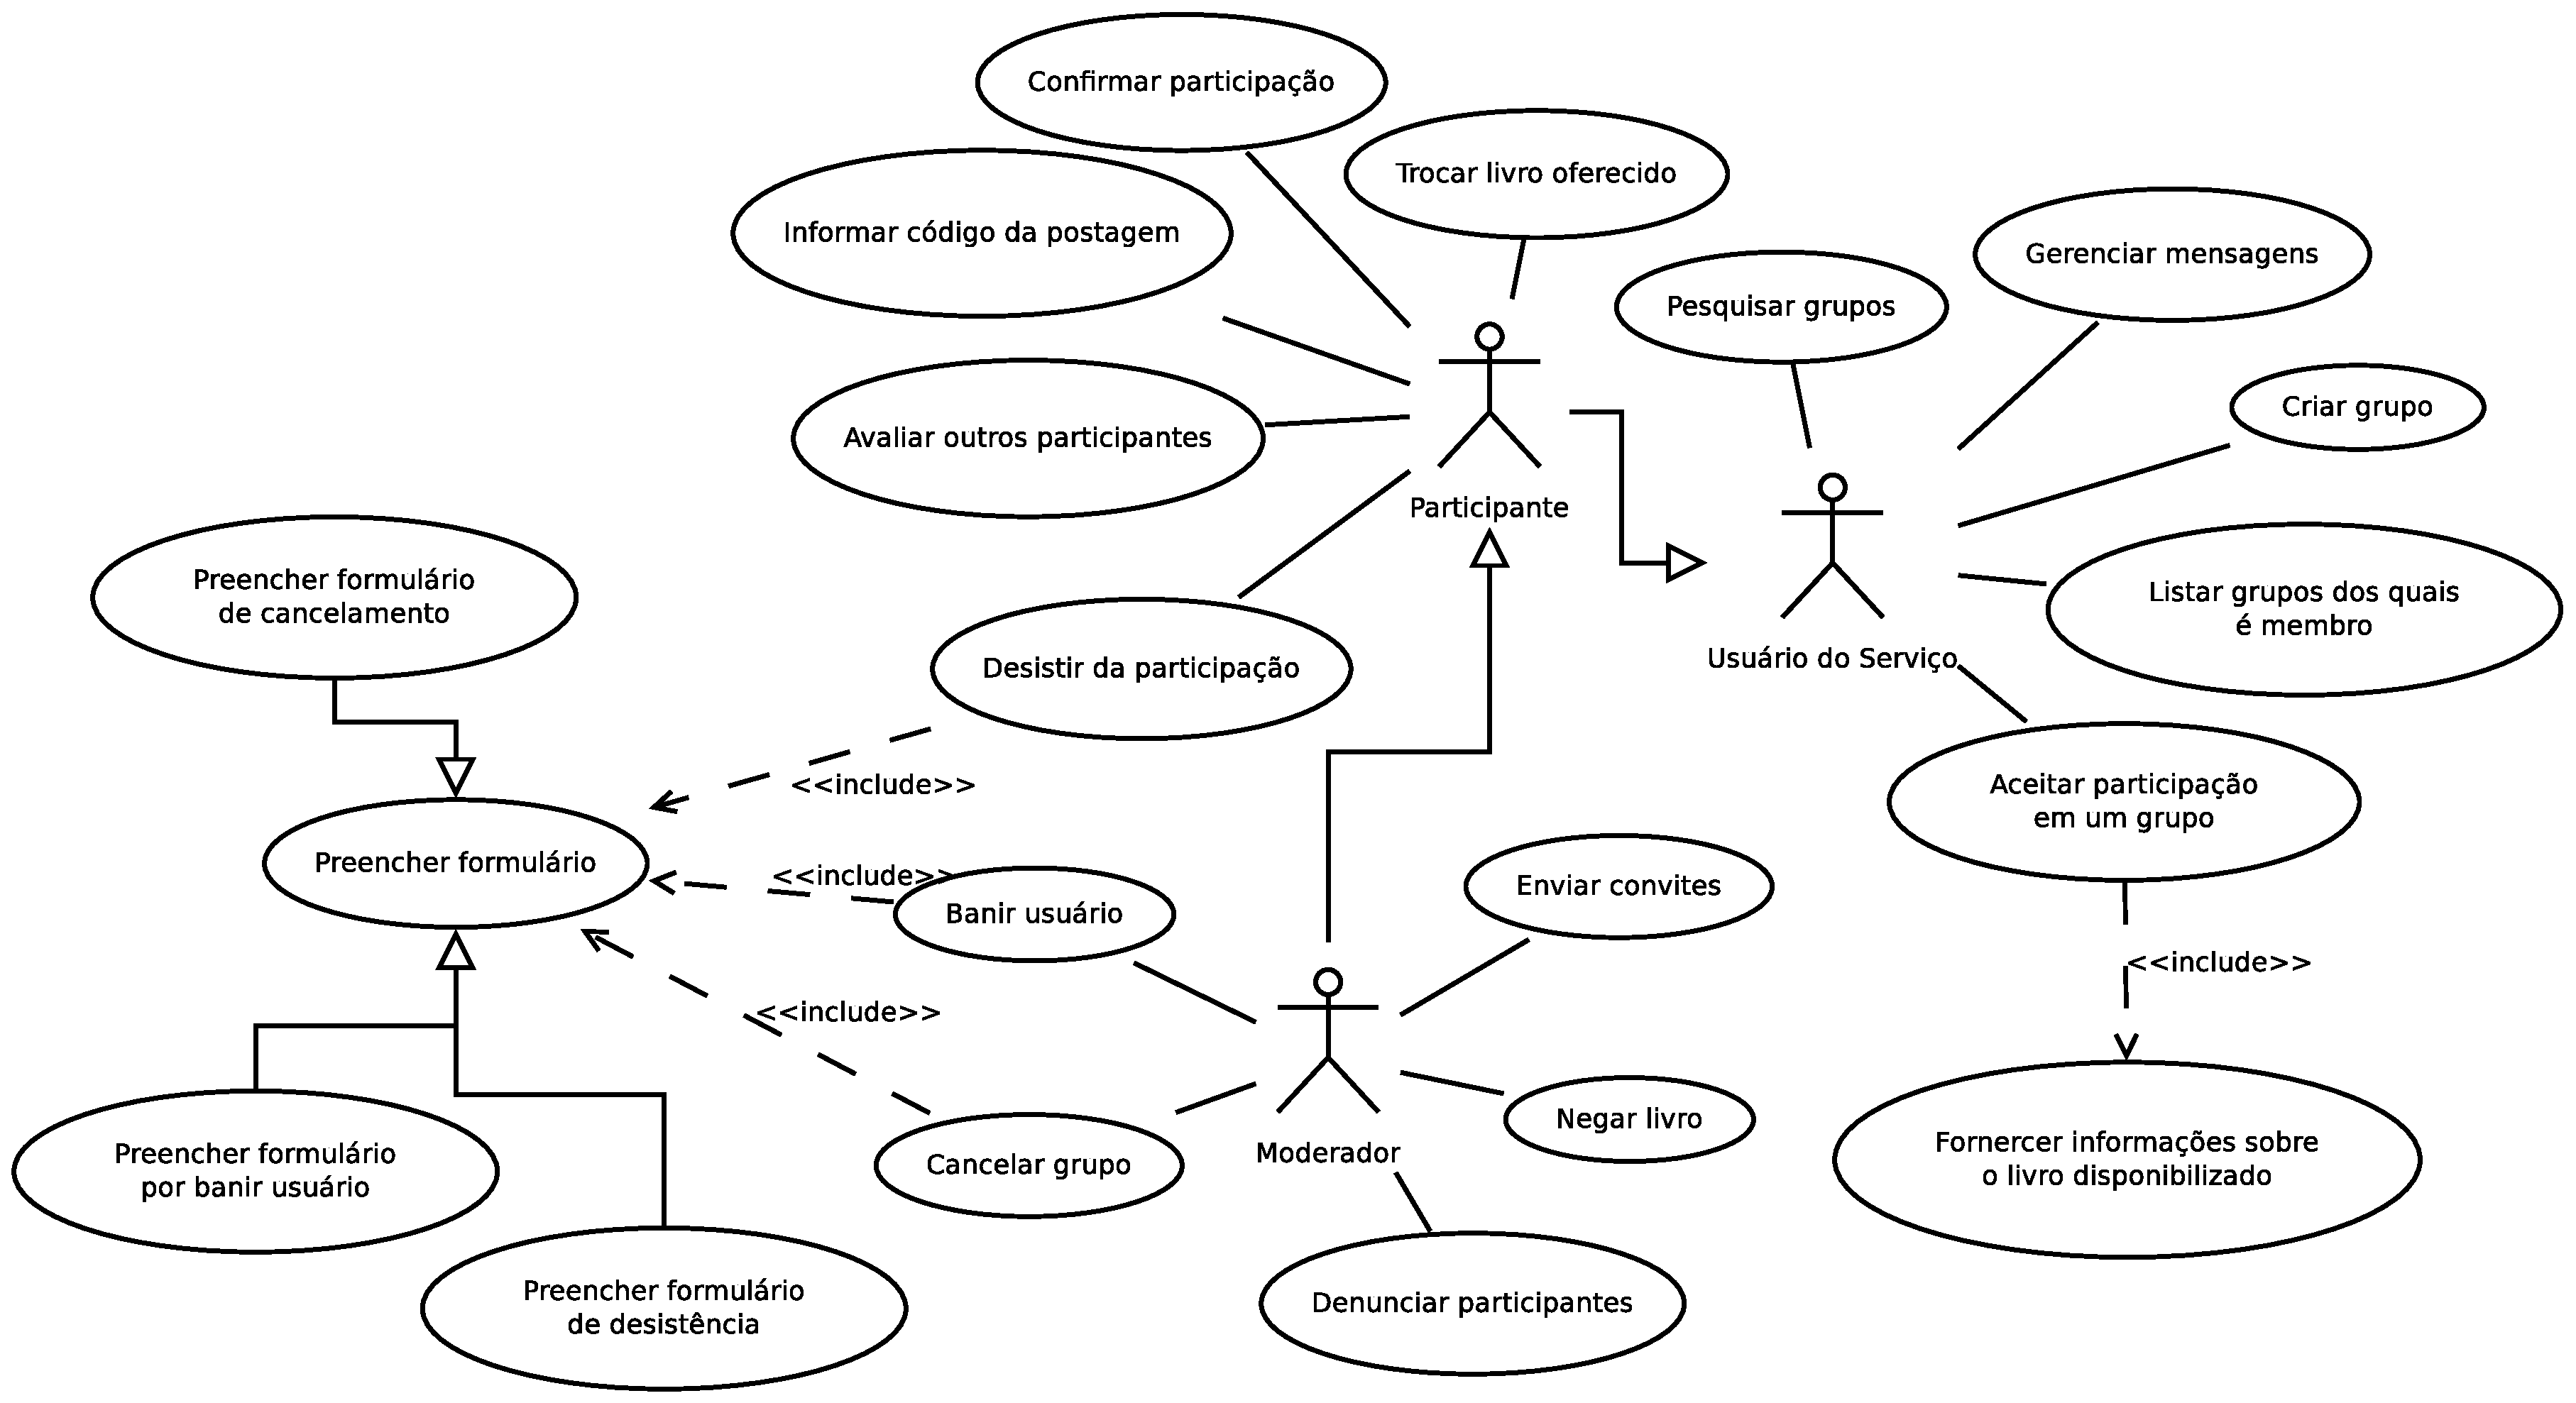
\includegraphics[width=\textwidth]{casosDeUso.eps}
  \caption{Diagrama de Casos de Uso}  
 \end{figure} 
\end{frame}

\end{document}
